%%%%%%%%%%%%%%%%%%%%%%%%%%%%%%%%%%%%%%%%%%%%%%%%%%%%%%%%%%%%%%%%%%%%%%%%%%%%%%%%%%
\begin{frame}[fragile]\frametitle{}
\begin{center}
{\Large Reflection Agents in LangGraph}

{\tiny (Ref: LangGraph Crash Course - Harish Neel)}

\end{center}
\end{frame}

%%%%%%%%%%%%%%%%%%%%%%%%%%%%%%%%%%%%%%%%%%%%%%%%%%%%%%%%%%%
\begin{frame}[fragile]\frametitle{Understanding Reflection - The Human Perspective}
      \begin{itemize}
        \item Reflection means looking at yourself or your actions, like viewing yourself in a mirror
        \item Self-reflection after giving a presentation - thinking about how it went
        \item Re-reading an email after writing to ensure clarity and correctness
        \item Considering if a decision was the right choice after making it
        \item Having a mirror in front of you to think about improvements
        \item Thinking about what you've done in the past and how to do better
        \item Foundation concept for understanding AI reflection patterns
      \end{itemize}
\end{frame}

%%%%%%%%%%%%%%%%%%%%%%%%%%%%%%%%%%%%%%%%%%%%%%%%%%%%%%%%%%%
\begin{frame}[fragile]\frametitle{What is a Reflection Agent Pattern?}
      \begin{itemize}
        \item AI system pattern that can look at its own outputs and improve them
        \item Similar to humans looking at themselves in a mirror and self-reflecting
        \item Makes AI systems better through iterative self-improvement
        \item Basic reflection agent system consists of two core components
        \item Generator agent - creates initial output or response
        \item Reflector agent - analyzes and critiques the generated output
        \item Both agents work together in a collaborative feedback loop
        \item Enables continuous improvement through multiple iterations
      \end{itemize}
\end{frame}

%%%%%%%%%%%%%%%%%%%%%%%%%%%%%%%%%%%%%%%%%%%%%%%%%%%%%%%%%%%
\begin{frame}[fragile]\frametitle{Practical Example: Viral Tweet Generator}
      \begin{itemize}
        \item Simple application demonstrating basic reflection agent pattern
        \item Start node initiates the process with user input topic
        \item Tweet Generation Agent creates initial tweet based on provided topic
        \item Conditional edge routes output to Tweet Critiquing Agent
        \item Tweet Critiquing Agent acts as critical reviewer of generated content
        \item Critique focuses on viral potential: length, CTAs, hooks, hashtags
        \item Feedback loop continues for 4-6 iterations for improvement
        \item Each iteration produces progressively better, more viral-worthy tweets
        \item Real-world application potential as product feature for customers
      \end{itemize}
\end{frame}

%%%%%%%%%%%%%%%%%%%%%%%%%%%%%%%%%%%%%%%%%%%%%%%%%%%%%%%%%%%
\begin{frame}[fragile]\frametitle{System 1 vs System 2: Traditional vs Reflection Patterns}
      \begin{itemize}
        \item \textbf{System 1 (Traditional):} One-shot prompt approach like ChatGPT/Claude
        \item Fast execution with immediate results
        \item Subconscious processing without active deep thinking
        \item Automatic response generation for everyday decisions
        \item More error-prone due to lack of reflection
        \item \textbf{System 2 (Reflection Pattern):} Two-agent collaborative approach
        \item Slower execution due to iterative feedback loops
        \item More conscious and effortful processing
        \item Better for complex decisions requiring precision
        \item Higher reliability through active thought-out responses
      \end{itemize}
\end{frame}

%%%%%%%%%%%%%%%%%%%%%%%%%%%%%%%%%%%%%%%%%%%%%%%%%%%%%%%%%%%
\begin{frame}[fragile]\frametitle{Reflection Loop Process Flow}
      \begin{itemize}
        \item Initial generation phase creates first response/output
        \item Reflection phase analyzes generated content critically
        \item Reflector identifies merits: what went right in the output
        \item Reflector identifies issues: what went wrong and needs improvement
        \item Critique feedback sent back to generator brain/agent
        \item Generator incorporates feedback to revise and improve output
        \item Loop repeats for predetermined number of iterations (n times)
        \item Final improved output delivered to user after iteration completion
        \item Process applicable beyond tweets to any content generation task
      \end{itemize}
\end{frame}

%%%%%%%%%%%%%%%%%%%%%%%%%%%%%%%%%%%%%%%%%%%%%%%%%%%%%%%%%%%
\begin{frame}[fragile]\frametitle{Three Types of Reflection Agents in LangGraph}
      \begin{itemize}
        \item \textbf{Basic Reflection Agents:} Foundation pattern with generator and reflector
        \item Reflector chain where reflector agent and generator agent work together
        \item Simple feedback loop for iterative improvement
        \item \textbf{Reflexion Agents:} Advanced pattern building on basic reflection
        \item Enhanced capabilities beyond basic reflection mechanisms
        \item \textbf{Language Agent Tree Search (LATS):} Most sophisticated approach
        \item Tree-based search methodology for complex decision making
        \item Recommended to master basic reflection first before advancing
        \item Progressive learning path from basic to advanced patterns
      \end{itemize}
\end{frame}

%%%%%%%%%%%%%%%%%%%%%%%%%%%%%%%%%%%%%%%%%%%%%%%%%%%%%%%%%%%
\begin{frame}[fragile]\frametitle{Introduction to LangGraph Message Graphs}
      \begin{itemize}
	\item MessageGraph orchestrates message flow between different nodes in a workflow
	\item Use MessageGraph for simple routing decisions and basic chatbot conversation flows
	\item Each node receives full list of previous messages as input
	\item Nodes can append new messages and return updated message list to next node
	\item Alternative StateGraph available for complex state management requirements
	\item MessageGraph maintains single shared message history across all chain operations
	\item System messages remain separate for each chain while sharing message history
	\item Perfect for reflection agent patterns where AI generates and critiques iteratively
	  \end{itemize}
\end{frame}

%%%%%%%%%%%%%%%%%%%%%%%%%%%%%%%%%%%%%%%%%%%%%%%%%%%%%%%%%%%
\begin{frame}[fragile]\frametitle{Building Graph Nodes and Structure}
      \begin{itemize}
	\item Create MessageGraph instance and define node constants (GENERATE, REFLECT)
	\item Generate node invokes generation chain with existing message state
	\item Reflect node uses reflection chain to critique previous AI responses
	\item Optional: Return human messages for reflection to improve readability and tracing
	\item Add nodes to graph using \texttt{graph.add\_node(name, function)}
	\item Set entry point explicitly - typically the generate node for first execution
	\item Should\_continue function controls iteration cycles based on message count
	\item Return 'END' when maximum iterations reached, otherwise continue to reflect
	\item Use conditional edges for branching logic (generate → should\_continue)
	\item Use simple edges for direct connections (reflect → generate)
	  \end{itemize}
\end{frame}

%%%%%%%%%%%%%%%%%%%%%%%%%%%%%%%%%%%%%%%%%%%%%%%%%%%%%%%%%%%
\begin{frame}[fragile]\frametitle{Basic Reflection Agents}

Define two chains first, then add them to graph

{\tiny (Ref: LangGraph Crash Course - Harish Neel)}

\begin{lstlisting}[basicstyle=\scriptsize\ttfamily]
from langchain_core.prompts import ChatPromptTemplate, MessagesPlaceholder
from langchain_google_genai import ChatGoogleGenerativeAI
from langchain_openai import ChatOpenAI

generation_prompt = ChatPromptTemplate.from_messages([("system",
            "You are a twitter techie influencer assistant tasked with writing excellent twitter posts.Generate the best twitter post possible for the user's request. If the user provides critique, respond with a revised version of your previous attempts.",),
        MessagesPlaceholder(variable_name="messages"),])

reflection_prompt = ChatPromptTemplate.from_messages([("system",
            "You are a viral twitter influencer grading a tweet. Generate critique and recommendations for the user's tweet. Always provide detailed recommendations, including requests for length, virality, style, etc.",),
		MessagesPlaceholder(variable_name="messages"), ])

llm = ChatOpenAI(model="gpt-4o")
generation_chain = generation_prompt | llm
reflection_chain = reflection_prompt | llm
  \end{lstlisting}
  
  

\end{frame}

%%%%%%%%%%%%%%%%%%%%%%%%%%%%%%%%%%%%%%%%%%%%%%%%%%%%%%%%%%%
\begin{frame}[fragile]\frametitle{Basic Reflection Agents}

Adding to graph

{\tiny (Ref: LangGraph Crash Course - Harish Neel)}

\begin{lstlisting}[basicstyle=\scriptsize\ttfamily]
from typing import List, Sequence
from dotenv import load_dotenv
from langchain_core.messages import BaseMessage, HumanMessage
from langgraph.graph import END, MessageGraph
from chains import generation_chain, reflection_chain

load_dotenv()

REFLECT = "reflect"
GENERATE = "generate"
graph = MessageGraph()

def generate_node(state):
    return generation_chain.invoke({
        "messages": state })

def reflect_node(messages):
    response = reflection_chain.invoke({
        "messages": messages})
    return [HumanMessage(content=response.content)]

graph.add_node(GENERATE, generate_node)
graph.add_node(REFLECT, reflect_node)
graph.set_entry_point(GENERATE)
\end{lstlisting}
  
  

\end{frame}


%%%%%%%%%%%%%%%%%%%%%%%%%%%%%%%%%%%%%%%%%%%%%%%%%%%%%%%%%%%
\begin{frame}[fragile]\frametitle{Basic Reflection Agents}

Adding to graph

{\tiny (Ref: LangGraph Crash Course - Harish Neel)}

\begin{lstlisting}[basicstyle=\scriptsize\ttfamily]
def should_continue(state):
    if (len(state) > 6):
        return END 
    return REFLECT


graph.add_conditional_edges(GENERATE, should_continue)
graph.add_edge(REFLECT, GENERATE)

app = graph.compile()

print(app.get_graph().draw_mermaid())
app.get_graph().print_ascii()

response = app.invoke(HumanMessage(content="AI Agents taking over content creation"))

print(response)

  \end{lstlisting}
  
  

\end{frame}

%%%%%%%%%%%%%%%%%%%%%%%%%%%%%%%%%%%%%%%%%%%%%%%%%%%%%%%%%%%%%%%%%%%%%%%%%%%%%%%%%%
\begin{frame}[fragile]\frametitle{}
\begin{center}
{\Large Structured LLM Outputs}
\end{center}
\end{frame}

%%%%%%%%%%%%%%%%%%%%%%%%%%%%%%%%%%%%%%%%%%%%%%%%%%%%%%%%%%%
\begin{frame}[fragile]\frametitle{Introduction to Structured Outputs}
      \begin{itemize}
	\item LLMs traditionally return unstructured string responses that are difficult to process programmatically
	\item Structured outputs allow models to return data matching specific schemas we define
	\item Essential for software engineering where we work with objects, JSON, and database-ready formats
	\item Instead of random strings, get organized data with exact properties for manipulation
	\item Multiple output formats supported: JSON, dictionary, string, YAML, HTML
	\item Example: Request a joke and receive setup, punchline, and rating in structured JSON format
	\item Enables seamless integration with databases and application workflows
	\item Critical foundation for building advanced agentic AI systems like reflexion agents
	\item Transforms LLM responses from text blobs into actionable data structures
	\item Makes LLM outputs suitable for automated processing and storage systems
	  \end{itemize}
\end{frame}

%%%%%%%%%%%%%%%%%%%%%%%%%%%%%%%%%%%%%%%%%%%%%%%%%%%%%%%%%%%
\begin{frame}[fragile]\frametitle{Pydantic Models for Structured Output}
      \begin{itemize}
	\item Pydantic is a Python library that defines data structures as blueprints for data validation
	\item Uses Python type hints (string, integer) to enforce correct data types automatically
	\item Define classes with required fields and descriptions for each property
	\item Integrated with LangChain using \texttt{with\_structured\_output()} method for LLM binding
	\item Works with any chat model (OpenAI, Groq, Llama) by simply swapping the model
	\item Internally converts Pydantic model into a tool that LLM must use exclusively
	\item Automatic validation ensures all properties are present with correct data types
	\item Throws errors automatically if validation fails, enabling fallback strategies
	\item LLM receives tool schema with property descriptions and required field specifications
	\item Response parsing and conversion handled automatically by LangChain framework
	  \end{itemize}
\end{frame}

%%%%%%%%%%%%%%%%%%%%%%%%%%%%%%%%%%%%%%%%%%%%%%%%%%%%%%%%%%%
\begin{frame}[fragile]\frametitle{Pydantic Model Implementation Example}
      \begin{itemize}
	\item Use \texttt{with\_structured\_output()} to bind model to LLM instance
	\item Tool choice parameter forces LLM to use only the specified schema
	\item Request payload includes tools array with function type and parameter specifications
	\item Response contains structured JSON matching exact schema requirements
	\item LangChain handles parsing, validation, and Pydantic model instantiation automatically
	\item Validation failures trigger automatic error handling for robust applications
	  \end{itemize}

\begin{lstlisting}[language=Python, basicstyle=\tiny]
from pydantic import BaseModel, Field

class Country(BaseModel):
    """Information about a country"""
    name: str = Field(description="Name of the country")
    language: str = Field(description="Language of the country")
    capital: str = Field(description="Capital of the country")

structured_llm = model.with_structured_output(Country)
response = structured_llm.invoke("Tell me about France")
\end{lstlisting}
\end{frame}

%%%%%%%%%%%%%%%%%%%%%%%%%%%%%%%%%%%%%%%%%%%%%%%%%%%%%%%%%%%
\begin{frame}[fragile]\frametitle{Alternative Methods: TypedDict and JSON Schema}
      \begin{itemize}
	\item TypedDict approach uses Python typing without Pydantic validation overhead
	\item Annotated class provides type hints, default values, and property descriptions
	\item JSON schema method offers direct schema definition without Python classes
	\item Schema requires title, description, properties, and required field specifications
	  \end{itemize}

\begin{lstlisting}[language=Python, basicstyle=\tiny]
# TypedDict approach
from typing import TypedDict, Annotated, Optional

class JokeDict(TypedDict):
    setup: Annotated[str, "Setup of the joke"]
    punchline: Annotated[str, "Punchline to the joke"]
    rating: Annotated[Optional[int], None, "Joke rating 1-10"]

# JSON Schema approach
joke_schema = {"title": "Joke","type": "object",
    "properties": {
        "setup": {"type": "string", "description": "Setup of joke"},
        "punchline": {"type": "string", "description": "Punchline"}
    },"required": ["setup", "punchline"]
}
\end{lstlisting}
\end{frame}


%%%%%%%%%%%%%%%%%%%%%%%%%%%%%%%%%%%%%%%%%%%%%%%%%%%%%%%%%%%%%%%%%%%%%%%%%%%%%%%%%%
\begin{frame}[fragile]\frametitle{}
\begin{center}
{\Large Reflexion Agent in LangGraph}
\end{center}
\end{frame}

%%%%%%%%%%%%%%%%%%%%%%%%%%%%%%%%%%%%%%%%%%%%%%%%%%%%%%%%%%%
\begin{frame}[fragile]\frametitle{Reflexion Agent System: Overview}
      \begin{itemize}
          \item Addresses drawbacks of basic reflection systems that lack grounding in live data
          \item Unlike reflection agents, reflexion agents fact-check with external data via API calls
          \item Combines self-critique with internet search capabilities for enriched content
          \item Generates citations and references from external sources during content creation
          \item Particularly useful for marketers writing blog posts requiring recent information
          \item Not limited to LLM training data cutoff dates like traditional reflection systems
          \item Iteratively improves content quality through multiple search-revise cycles
          \item Enables creation of well-researched, factually grounded content with live data
          \item Prevents hallucinations by validating information against current sources
          \item Supports episodic memory for context-aware, personalized interactions over time
      \end{itemize}
\end{frame}

%%%%%%%%%%%%%%%%%%%%%%%%%%%%%%%%%%%%%%%%%%%%%%%%%%%%%%%%%%%%%%%%%%%%%%%%%%%%%%%%%%
\begin{frame}[fragile]\frametitle{Reflexion Agent}

\begin{center}
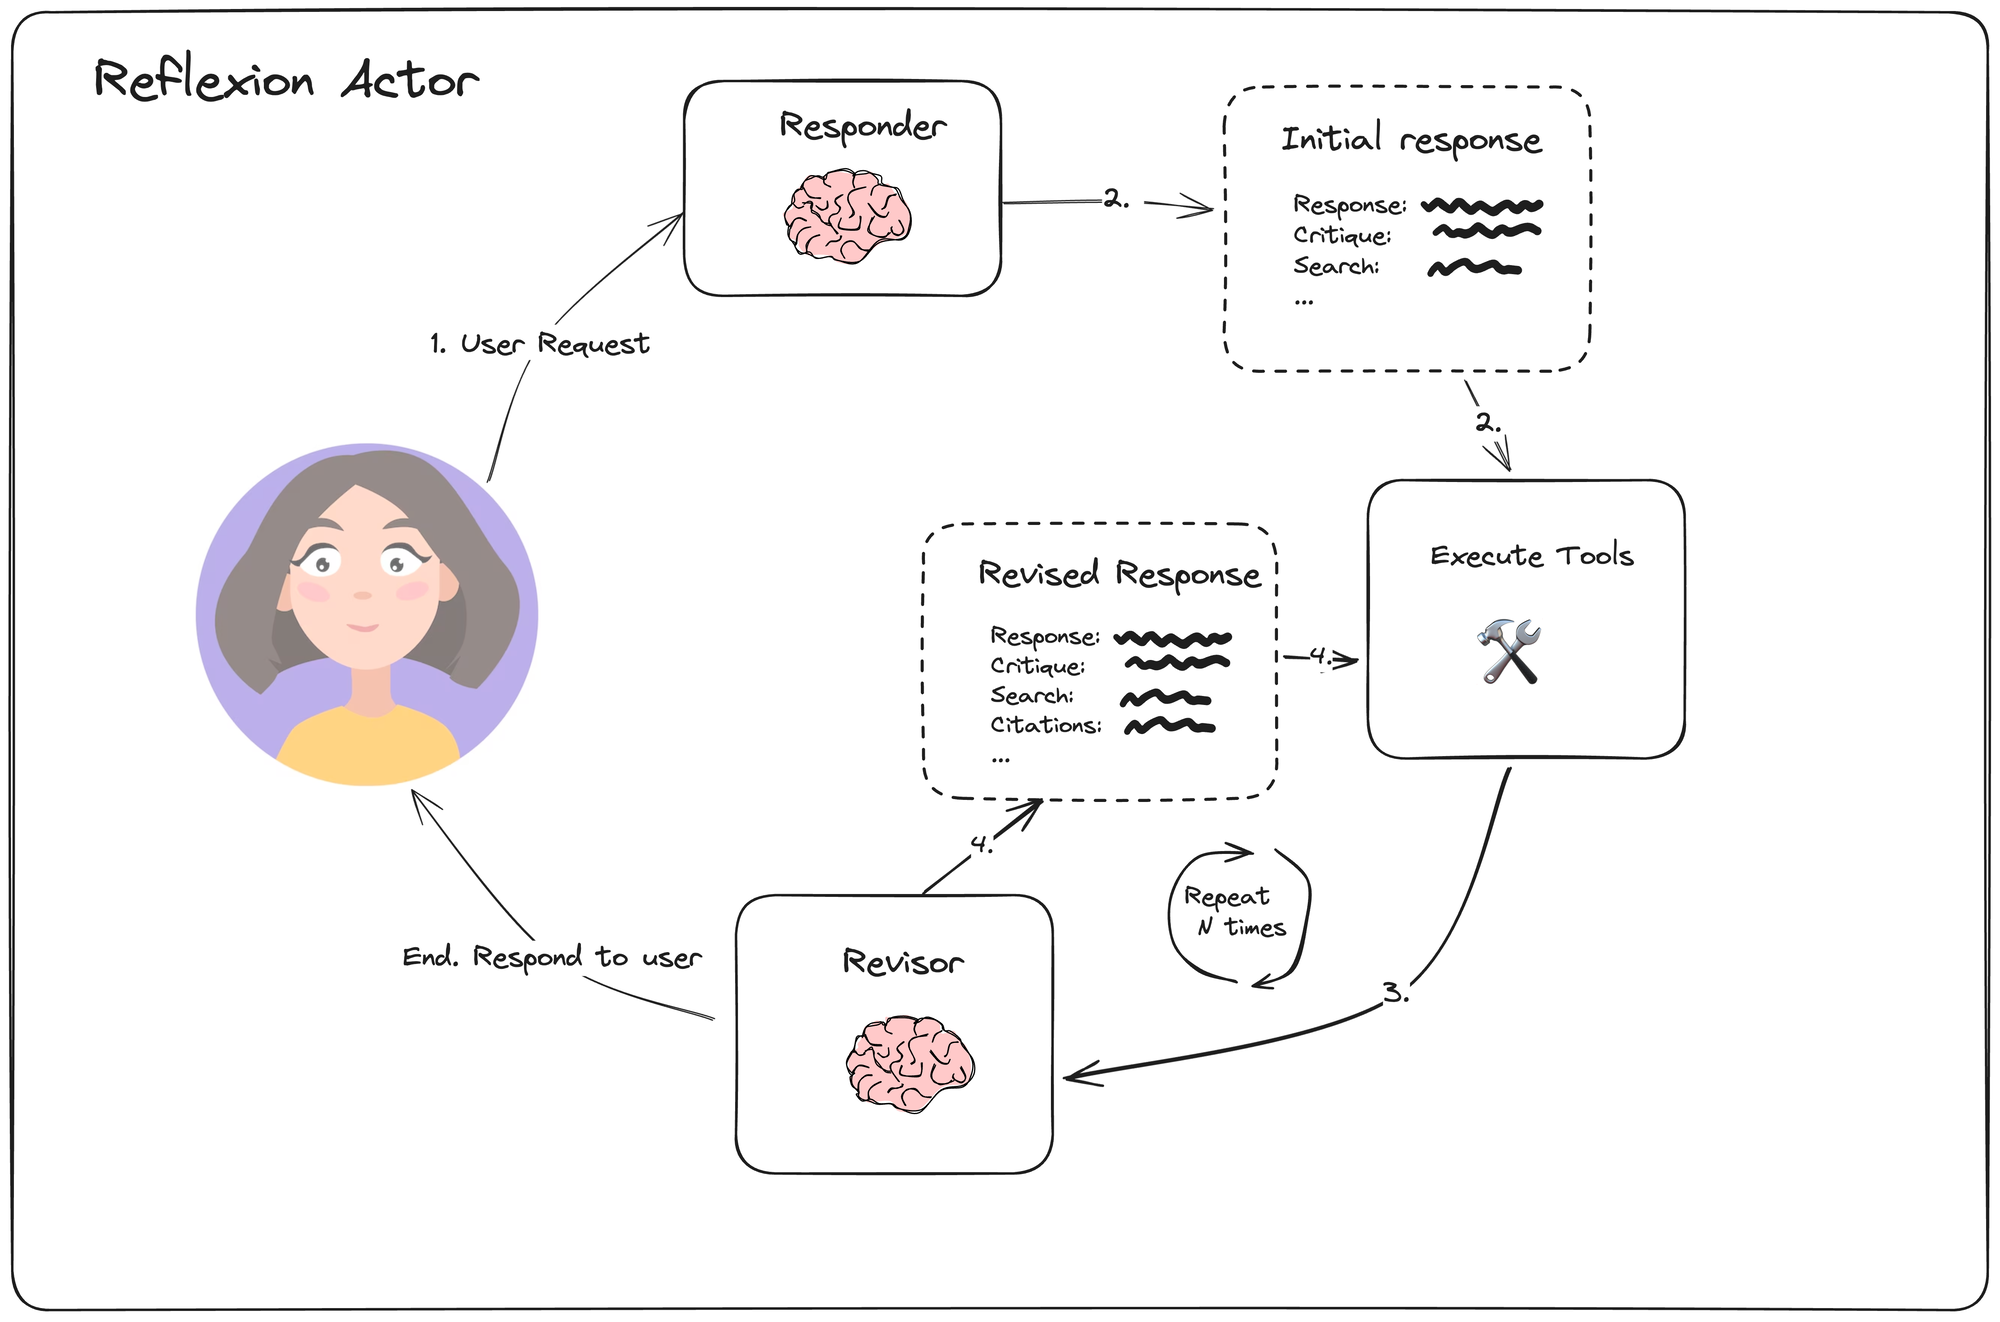
\includegraphics[width=0.8\linewidth,keepaspectratio]{langgraph11}

{\tiny (Ref: LangGraph Crash Course - Harish Neel)}

\end{center}	  


\end{frame}


%%%%%%%%%%%%%%%%%%%%%%%%%%%%%%%%%%%%%%%%%%%%%%%%%%%%%%%%%%%
\begin{frame}[fragile]\frametitle{Core Components Architecture}
      \begin{itemize}
          \item \textbf{Actor Agent:} Main driver that orchestrates all subcomponents and processes
          \item \textbf{Responder Agent:} Generates initial response with self-reflection capabilities
          \item \textbf{Revisor Agent:} Creates revised responses based on new external data
          \item \textbf{Tools/Tool Execution:} Handles API calls, primarily internet search functionality
          \item \textbf{Episodic Memory:} Recalls specific past interactions and experiences for context
          \item Actor contains all subcomponents: responder, revisor, and execute tools modules
          \item System operates through iterative loops of generation, search, and revision
          \item Each component has specific responsibilities within the overall workflow
          \item Tool execution primarily uses Tavily Search for gathering live internet data
          \item Architecture designed for modularity and extensibility with additional tools
      \end{itemize}
\end{frame}

%%%%%%%%%%%%%%%%%%%%%%%%%%%%%%%%%%%%%%%%%%%%%%%%%%%%%%%%%%%
\begin{frame}[fragile]\frametitle{Workflow and Data Flow}
      \begin{itemize}
          \item User request goes to responder agent for initial content generation
          \item Responder outputs JSON with response, critique, and suggested search keywords
          \item Execute tools component searches internet using suggested keywords via Tavily
          \item Search results combined with initial response fed to revisor agent
          \item Revisor generates revised response with updated critique and citations
          \item Citations added to reference external sources used in content creation
          \item Process iterates: revised search terms trigger new searches and revisions
          \item Each iteration enriches content with more recent, relevant information
          \item Content length maintained (e.g., 250 words) while improving quality and accuracy
          \item Final output returned to user after multiple refinement cycles complete
      \end{itemize}
\end{frame}

%%%%%%%%%%%%%%%%%%%%%%%%%%%%%%%%%%%%%%%%%%%%%%%%%%%%%%%%%%%
\begin{frame}[fragile]\frametitle{JSON Response Structure Example}
      \begin{itemize}
          \item Responder agent outputs structured JSON with three main properties
          \item \textbf{Response:} Contains the initial generated content (e.g., 250-word blog post)
          \item \textbf{Critique:} Self-assessment identifying areas for improvement in content
          \item \textbf{Search Terms:} Keywords suggested for gathering additional relevant information
          \item Revisor agent extends structure with additional citation property
          \item \textbf{Citations:} References to external sources with URLs and factual backing
          \item Revised versions update all properties: response, critique, search terms, citations
          \item Structure enables systematic improvement through multiple iterations
          \item JSON format facilitates programmatic processing and integration with LangGraph
          \item Supports grounding of content claims with verifiable external sources
      \end{itemize}
\end{frame}


%%%%%%%%%%%%%%%%%%%%%%%%%%%%%%%%%%%%%%%%%%%%%%%%%%%%%%%%%%%%%%%%%%%%%%%%%%%%%%%%%%
\begin{frame}[fragile]\frametitle{}
\begin{center}
{\Large Advanced Concepts in LangGraph}
\end{center}
\end{frame}

%%%%%%%%%%%%%%%%%%%%%%%%%%%%%%%%%%%%%%%%%%%%%%%%%%%%%%%%%%%
\begin{frame}[fragile]\frametitle{Advanced Conditional Edges}

Conditional edges allow to dynamically decide the execution flow based on the state.

      \begin{lstlisting}[language=Python, basicstyle=\tiny]
from typing import List, Dict, Literal
from pydantic import BaseModel

class AgentState(BaseModel):
    messages: List[Dict[str, str]] = []
    current_input: str = ""
    tools_output: Dict[str, str] = {}
    status: str = "RUNNING"
    error_count: int = 0

def route_by_status(state: AgentState) -> Literal["process", "retry", "error", "end"]:
    if state.status == "SUCCESS":
        return "end"
    elif state.status == "ERROR":
        if state.error_count >= 3:
            return "error"
        return "retry"
    elif state.status == "NEED_TOOL":
        return "process"
    return "process"

workflow.add_conditional_edges(
    "check_status",
    route_by_status,
    {"process": "execute_tool", "retry": "retry_handler", 
     "error": "error_handler", "end": END}
)
      \end{lstlisting}
\end{frame}

%%%%%%%%%%%%%%%%%%%%%%%%%%%%%%%%%%%%%%%%%%%%%%%%%%%%%%%%%%%
\begin{frame}[fragile]\frametitle{Parallel Execution in LangGraph}
Supports parallel execution of multiple nodes, which is particularly useful for handling complex tasks:

      \begin{lstlisting}[language=Python, basicstyle=\tiny]
async def parallel_tools_execution(state: AgentState) -> AgentState:
    """Parallel execution of multiple tools"""
    tools = identify_required_tools(state.current_input)

    async def execute_tool(tool):
        result = await tool.ainvoke(state.current_input)
        return {tool.name: result}

    # Execute all tools in parallel
    results = await asyncio.gather(*[execute_tool(tool) for tool in tools])

    # Merge results
    tools_output = {}
    for result in results:
        tools_output.update(result)

    return AgentState(
        messages=state.messages,
        current_input=state.current_input,
        tools_output=tools_output,
        status="SUCCESS"
    )
      \end{lstlisting}
\end{frame}


%%%%%%%%%%%%%%%%%%%%%%%%%%%%%%%%%%%%%%%%%%%%%%%%%%%%%%%%%%%
\begin{frame}[fragile]\frametitle{ReACT Architecture Introduction}
      \begin{itemize}
        \item ReACT (Reasoning and Acting) combines reasoning and acting capabilities
        \item Agent solves problems through continuous cycle: Reason → Act → Observe
        \item Flexible response to complex tasks using external tools
        \item Enhanced capabilities through tool integration
        \item LangGraph provides pre-built ReACT agents
        \item Supports Google search, DALL-E image generation, and more
        \item Easy implementation with create\_react\_agent function
        \item Suitable for dynamic problem-solving scenarios
      \end{itemize}
\end{frame}

%%%%%%%%%%%%%%%%%%%%%%%%%%%%%%%%%%%%%%%%%%%%%%%%%%%%%%%%%%%
\begin{frame}[fragile]\frametitle{ReACT Agent Implementation}
      \begin{lstlisting}[language=Python, basicstyle=\tiny]
import dotenv
from langchain_community.tools import GoogleSerperRun
from langchain_community.tools.openai_dalle_image_generation import OpenAIDALLEImageGenerationTool
from langchain_openai import ChatOpenAI
from langgraph.prebuilt.chat_agent_executor import create_react_agent

dotenv.load_dotenv()

# Define Tools and Parameter Schemas
google_serper = GoogleSerperRun(
    name="google_serper",
    description="A low-cost Google search API for current events",
    args_schema=GoogleSerperArgsSchema,
    api_wrapper=GoogleSerperAPIWrapper(),
)

dalle = OpenAIDALLEImageGenerationTool(
    name="openai_dalle",
    api_wrapper=DallEAPIWrapper(model="dall-e-3"),
    args_schema=DallEArgsSchema,
)

tools = [google_serper, dalle]
model = ChatOpenAI(model="gpt-4o-mini", temperature=0)

# Create ReACT agent
agent = create_react_agent(model=model, tools=tools)

# Usage
result = agent.invoke({"messages": [("human", "Help me draw a shark flying in the sky")]})
      \end{lstlisting}
\end{frame}

%%%%%%%%%%%%%%%%%%%%%%%%%%%%%%%%%%%%%%%%%%%%%%%%%%%%%%%%%%%
\begin{frame}[fragile]\frametitle{Analysis of Results}

      \begin{itemize}
        \item the agent will first understand the task requirements and then decide to use the DALL-E tool to generate an image. 
		\item It will generate a detailed image description and then call the DALL-E API to create the image. 
        \item Finally, it will return the generated image URL along with a brief description.
		\item The output might look like this:
      \end{itemize}



      \begin{lstlisting}[language=Python, basicstyle=\tiny]
{
    "messages": [
        HumanMessage(content='Help me draw a picture of a shark flying in the sky'),
        AIMessage(content='', additional_kwargs={'tool_calls': [...]}),
        ToolMessage(content='https://dalleproduse.blob.core.windows.net/...'),
        AIMessage(content='Here is the image you requested: a picture of a shark flying in the sky. You can view the image by clicking the link below.\n\n![Shark flying in the sky](https://dalleproduse.blob.core.windows.net/...)')
    ]
}
      \end{lstlisting}
\end{frame}




%%%%%%%%%%%%%%%%%%%%%%%%%%%%%%%%%%%%%%%%%%%%%%%%%%%%%%%%%%%
\begin{frame}[fragile]\frametitle{Message Management in LangGraph}
      \begin{itemize}
        \item Message accumulation can lead to performance issues
        \item delete\_messages function removes processed messages
        \item Filtering techniques control message flow
        \item Conditional edges for message routing
        \item Time-based and quantity-based pruning strategies
        \item Essential for long-running applications
        \item Maintains conversation clarity and focus
        \item Improves overall system performance
      \end{itemize}
\end{frame}

%%%%%%%%%%%%%%%%%%%%%%%%%%%%%%%%%%%%%%%%%%%%%%%%%%%%%%%%%%%
\begin{frame}[fragile]\frametitle{Message Deletion and Filtering}

Can delete messages based on specified conditions. This function can be used in the nodes of the graph, especially after processing certain messages.

      \begin{lstlisting}[language=Python, basicstyle=\tiny]
from langgraph.prebuilt import ToolMessage, delete_messages

def process_and_delete(state):
    # Processing logic
    # Delete processed messages
    state = delete_messages(state, lambda x: isinstance(x, ToolMessage))
    return state

def filter_messages(state):
    filtered_messages = [msg for msg in state['messages'] 
                        if not isinstance(msg, ToolMessage)]
    return {"messages": filtered_messages}

def keep_latest_messages(state, max_messages=50):
    return {"messages": state['messages'][-max_messages:]}

# Time-based pruning
from datetime import datetime, timedelta

def prune_old_messages(state):
    current_time = datetime.now()
    recent_messages = [msg for msg in state['messages'] 
                      if current_time - msg.timestamp < timedelta(hours=1)]
    return {"messages": recent_messages}
      \end{lstlisting}
\end{frame}

%%%%%%%%%%%%%%%%%%%%%%%%%%%%%%%%%%%%%%%%%%%%%%%%%%%%%%%%%%%
\begin{frame}[fragile]\frametitle{Checkpoint Mechanism}
      \begin{itemize}
        \item Checkpoints are snapshots during graph execution
        \item Enable pause and resume functionality for long-running tasks
        \item Useful for processes requiring human intervention
        \item Support state rollback to previous points
        \item Allow data modification at checkpoints
        \item Use thread\_id and thread\_ts for unique identification
        \item Retrieve last state and execution history
        \item Essential for resumable AI applications
      \end{itemize}
\end{frame}

%%%%%%%%%%%%%%%%%%%%%%%%%%%%%%%%%%%%%%%%%%%%%%%%%%%%%%%%%%%
\begin{frame}[fragile]\frametitle{Checkpoint Implementation}
      \begin{lstlisting}[language=Python, basicstyle=\tiny]
from langgraph.checkpoint import create_checkpoint, load_checkpoint

def process_with_checkpoint(state):
    # Processing logic
    # Create a checkpoint
    checkpoint = create_checkpoint(state)
    return {"checkpoint": checkpoint, "state": state}

def resume_from_checkpoint(checkpoint):
    state = load_checkpoint(checkpoint)
    # Continue processing
    return state

# Using checkpoints in practice
def summarize_and_prune(state):
    summary = summarize_conversation(state['messages'])
    new_messages = state['messages'][-5:]
    new_messages.append(ToolMessage(content=summary))
    state['messages'] = new_messages
    
    # Create checkpoint
    checkpoint = create_checkpoint(state)
    state['checkpoint'] = checkpoint
    return state

# Retrieve state and history
graph.get_state(config)  # Get last saved state
graph.get_state_history(config)  # Get all saved states
      \end{lstlisting}
\end{frame}

%%%%%%%%%%%%%%%%%%%%%%%%%%%%%%%%%%%%%%%%%%%%%%%%%%%%%%%%%%%
\begin{frame}[fragile]\frametitle{Human-in-the-Loop Interaction}
      \begin{itemize}
        \item Allows human participation in AI decision-making process
        \item Callback functions obtain human input during execution
        \item Conditional branching determines when human intervention needed
        \item Confidence-based routing for automatic vs manual processing
        \item Enhanced system reliability through human oversight
        \item Flexible interaction control mechanisms
        \item Improves decision quality in critical scenarios
        \item Supports collaborative human-AI workflows
      \end{itemize}
\end{frame}

%%%%%%%%%%%%%%%%%%%%%%%%%%%%%%%%%%%%%%%%%%%%%%%%%%%%%%%%%%%
\begin{frame}[fragile]\frametitle{Human Interaction Implementation}
      \begin{lstlisting}[language=Python, basicstyle=\tiny]
def human_input_node(state):
    # Display current state to user
    print("Current state:", state)
    # Get user input
    user_input = input("Please provide your input: ")
    # Update state
    state['user_input'] = user_input
    return state

def check_confidence(state):
    if state['confidence'] < 0.8:
        return "human_input"
    else:
        return "auto_process"

def human_intervention(state):
    print("Current conversation:", state['messages'])
    human_response = input("Please provide assistance: ")
    state['messages'].append(HumanMessage(content=human_response))
    return state

# Add conditional routing
graph.add_conditional_edges("process_query", {
    "human_intervention": lambda s: s['confidence'] < 0.8,
    "auto_process": lambda s: s['confidence'] >= 0.8
})
      \end{lstlisting}
\end{frame}

%%%%%%%%%%%%%%%%%%%%%%%%%%%%%%%%%%%%%%%%%%%%%%%%%%%%%%%%%%%
\begin{frame}[fragile]\frametitle{Subgraph Architecture}
A subgraph is essentially a complete graph structure that can be used as a node in a larger graph structure. 

      \begin{itemize}
        \item Break complex workflows into manageable components
        \item Modular design enhances code reusability
        \item Independent subgraphs improve maintainability
        \item Easy testing and debugging of individual components
        \item Scalable architecture for adding new features
        \item Encapsulate complex logic in reusable modules
        \item Support composition and interaction between subgraphs
        \item Enable hierarchical workflow organization
      \end{itemize}
\end{frame}

%%%%%%%%%%%%%%%%%%%%%%%%%%%%%%%%%%%%%%%%%%%%%%%%%%%%%%%%%%%
\begin{frame}[fragile]\frametitle{Subgraph Implementation}

Creating a Basic Subgraph

\begin{lstlisting}[language=Python, basicstyle=\tiny]
from langgraph.graph import SubGraph, Graph

class ContentGenerationSubGraph(SubGraph):
    def build(self) -> Graph:
        graph = Graph()
        
        def generate_content(state):
            # Content generation logic
            return state
            
        def review_content(state):
            # Content review logic
            return state
\end{lstlisting}
\end{frame}

%%%%%%%%%%%%%%%%%%%%%%%%%%%%%%%%%%%%%%%%%%%%%%%%%%%%%%%%%%%
\begin{frame}[fragile]\frametitle{Subgraph Implementation}

State Management in Subgraph

\begin{lstlisting}[language=Python, basicstyle=\tiny]
class AnalyticsSubGraph(SubGraph):
    def build(self) -> Graph:
        graph = Graph()

        def process_analytics(state):
            # Ensure the state contains necessary keys
            if 'metrics' not in state:
                state['metrics'] = {}
            # Process analytics data
            state['metrics']['engagement'] = calculate_engagement(state)
            return state

        graph.add_node("analytics", process_analytics)
        return graph
\end{lstlisting}
\end{frame}


%%%%%%%%%%%%%%%%%%%%%%%%%%%%%%%%%%%%%%%%%%%%%%%%%%%%%%%%%%%
\begin{frame}[fragile]\frametitle{Subgraph Implementation}

Using Subgraphs in the Main Graph

\begin{lstlisting}[language=Python, basicstyle=\tiny]
def create_marketing_workflow():
    main_graph = Graph()
    # Instantiate subgraphs
    content_graph = ContentGenerationSubGraph()
    analytics_graph = AnalyticsSubGraph()
    # Add subgraphs to the main graph
    main_graph.add_node("content", content_graph)
    main_graph.add_node("analytics", analytics_graph)
    # Connect subgraphs
    main_graph.add_edge("content", "analytics")
    return main_graph
\end{lstlisting}
\end{frame}

%%%%%%%%%%%%%%%%%%%%%%%%%%%%%%%%%%%%%%%%%%%%%%%%%%%%%%%%%%%
\begin{frame}[fragile]\frametitle{Subgraph Implementation}

Data Passing Between Subgraphs

\begin{lstlisting}[language=Python, basicstyle=\tiny]
class DataProcessingSubGraph(SubGraph):
    def build(self) -> Graph:
        graph = Graph()

        def prepare_data(state):
            # Prepare data for use by other subgraphs
            state['processed_data'] = {
                'content_type': state['raw_data']['type'],
                'metrics': state['raw_data']['metrics'],
                'timestamp': datetime.now()
            }
            return state

        graph.add_node("prepare", prepare_data)
        return graph
\end{lstlisting}
\end{frame}

%%%%%%%%%%%%%%%%%%%%%%%%%%%%%%%%%%%%%%%%%%%%%%%%%%%%%%%%%%%
\begin{frame}[fragile]\frametitle{Practical Case: Implementation of Marketing Agent}

Content Generation Subgraph

\begin{lstlisting}[language=Python, basicstyle=\tiny]
class ContentCreationSubGraph(SubGraph):
    def build(self) -> Graph:
        graph = Graph()

        def generate_content(state):
            prompt = f"""
            Target Audience: {state['audience']}
            Platform: {state['platform']}
            Campaign Goal: {state['goal']}
            """
            # Use LLM to generate content
            content = generate_with_llm(prompt)
            state['generated_content'] = content
            return state

        def optimize_content(state):
            # Optimize content according to platform characteristics
            optimized = optimize_for_platform(state['generated_content'], state['platform'])
            state['final_content'] = optimized
            return state

        graph.add_node("generate", generate_content)
        graph.add_node("optimize", optimize_content)
        graph.add_edge("generate", "optimize")
        return graph
\end{lstlisting}
\end{frame}

%%%%%%%%%%%%%%%%%%%%%%%%%%%%%%%%%%%%%%%%%%%%%%%%%%%%%%%%%%%
\begin{frame}[fragile]\frametitle{Practical Case: Implementation of Marketing Agent}

Analytics Subgraph

\begin{lstlisting}[language=Python, basicstyle=\tiny]
class AnalyticsSubGraph(SubGraph):
    def build(self) -> Graph:
        graph = Graph()

        def analyze_performance(state):
            metrics = calculate_metrics(state['final_content'])
            state['analytics'] = {
                'engagement_score': metrics['engagement'],
                'reach_prediction': metrics['reach'],
                'conversion_estimate': metrics['conversion']
            }
            return state

        def generate_recommendations(state):
            recommendations = generate_improvements(state['analytics'], state['goal'])
            state['recommendations'] = recommendations
            return state

        graph.add_node("analyze", analyze_performance)
        graph.add_node("recommend", generate_recommendations)
        graph.add_edge("analyze", "recommend")
        return graph
\end{lstlisting}
\end{frame}

%%%%%%%%%%%%%%%%%%%%%%%%%%%%%%%%%%%%%%%%%%%%%%%%%%%%%%%%%%%
\begin{frame}[fragile]\frametitle{Practical Case: Implementation of Marketing Agent}

Main Workflow

\begin{lstlisting}[language=Python, basicstyle=\tiny]
def create_marketing_agent():
    main_graph = Graph()
    # Instantiate subgraphs
    content_graph = ContentCreationSubGraph()
    analytics_graph = AnalyticsSubGraph()

    # Add configuration node
    def setup_campaign(state):
        # Initialize marketing campaign configuration
        if 'config' not in state:
            state['config'] = {
                'audience': state.get('audience', 'general'),
                'platform': state.get('platform', 'twitter'),
                'goal': state.get('goal', 'engagement')
            }
        return state

    main_graph.add_node("setup", setup_campaign)
    main_graph.add_node("content", content_graph)
    main_graph.add_node("analytics", analytics_graph)
    # Build workflow
    main_graph.add_edge("setup", "content")
    main_graph.add_edge("content", "analytics")
    return main_graph
\end{lstlisting}
\end{frame}

%%%%%%%%%%%%%%%%%%%%%%%%%%%%%%%%%%%%%%%%%%%%%%%%%%%%%%%%%%%
\begin{frame}[fragile]\frametitle{Subgraph Best Practices and Considerations}

      \begin{itemize}
        \item Design Principles for Subgraphs
		      \begin{itemize}
				\item Keep subgraph functionality singular
				\item Ensure clear input and output interfaces
				\item Properly handle state passing
			  \end{itemize}
				
        \item Performance Considerations
		      \begin{itemize}
				\item Avoid frequent large data transfers between subgraphs
				\item Design state storage structures reasonably
				\item Consider asynchronous processing needs
			  \end{itemize}
				
        \item Error Handling
		      \begin{itemize}
				\item Implement error handling within subgraphs
				\item Provide clear error messages
				\item Ensure state consistency
			  \end{itemize}
				
      \end{itemize}
\end{frame}

%%%%%%%%%%%%%%%%%%%%%%%%%%%%%%%%%%%%%%%%%%%%%%%%%%%%%%%%%%%
\begin{frame}[fragile]\frametitle{Data State and Induction Functions}
      \begin{itemize}
        \item Default behavior overwrites original data completely
        \item Manual state retrieval and update prevents data loss
        \item Induction functions provide automatic data accumulation
        \item Annotated wrapper simplifies state management
        \item Independent node execution without state conflicts
        \item Type hints improve code clarity and debugging
        \item Simplified node modification when updating structures
        \item Enhanced data consistency across workflow execution
      \end{itemize}
\end{frame}

%%%%%%%%%%%%%%%%%%%%%%%%%%%%%%%%%%%%%%%%%%%%%%%%%%%%%%%%%%%
\begin{frame}[fragile]\frametitle{Induction Functions Example}

Understanding how data states are handled in LangGraph is crucial. By default, the dictionary data returned by nodes will overwrite the original data, which may lead to unexpected results. For example:

\begin{lstlisting}[language=Python, basicstyle=\tiny]
from typing import TypedDict, Annotated

# Problem: Default behavior overwrites data
class MyState(TypedDict):
    messages: list

def fn1(state: MyState):
    return {"messages": [4]}

r = graph.invoke({"messages": [1, 2, 3]})
# Result: {"messages": [4]} instead of [1,2,3,4]

\end{lstlisting}
\end{frame}


%%%%%%%%%%%%%%%%%%%%%%%%%%%%%%%%%%%%%%%%%%%%%%%%%%%%%%%%%%%
\begin{frame}[fragile]\frametitle{Induction Functions Example}

To solve this problem, LangGraph provides two methods for accumulating data:

\begin{lstlisting}[language=Python, basicstyle=\tiny]

# Manually retrieve and update the original state:
  def fn1(state: MyState):
      old = state.get("messages", [])
      return {"messages": old + [4]}

	
# Use LangGraph's Annotated wrapper and induction functions:
def concat_lists(original: list, new: list) -> list:
    return original + new

class MyState(TypedDict):
    messages: Annotated[list, concat_lists]

def fn1(state: MyState):
    return {"messages": [4]}

r = graph.invoke({"messages": [1, 2, 3]})
# Result: {'messages': [1, 2, 3, 4]}
      \end{lstlisting}
\end{frame}

%%%%%%%%%%%%%%%%%%%%%%%%%%%%%%%%%%%%%%%%%%%%%%%%%%%%%%%%%%%
\begin{frame}[fragile]\frametitle{Parallel Node Execution}
      \begin{itemize}
        \item END node signifies route termination, not graph termination
        \item Nodes at same level execute in parallel
        \item Execution order is uncertain in parallel execution
        \item Control flow by adjusting node connections
        \item Important for understanding graph execution model
        \item Optimize performance through parallel processing
        \item Design considerations for concurrent operations
        \item Manage dependencies between parallel nodes
      \end{itemize}
	  
\begin{lstlisting}	  
graph.add_edge(["left1", "right3"], "merge")	
\end{lstlisting}
\end{frame}

%%%%%%%%%%%%%%%%%%%%%%%%%%%%%%%%%%%%%%%%%%%%%%%%%%%%%%%%%%%
\begin{frame}[fragile]\frametitle{CheckPoint Mechanism}

Checkpoints can be seen as a storage medium for recording node states. Key features include:
      \begin{itemize}
        \item Retrieving the last state and history
        \item Supports state rollback
        \item Allows data modification
        \item Uses thread\_id and thread\_ts to uniquely locate archives
      \end{itemize}
	  
\begin{lstlisting}	  
  graph.get_state(config)  # Get the last saved state
  graph.get_state_history(config)  # Get the list of all saved states	
\end{lstlisting}
\end{frame}

%%%%%%%%%%%%%%%%%%%%%%%%%%%%%%%%%%%%%%%%%%%%%%%%%%%%%%%%%%%
\begin{frame}[fragile]\frametitle{Best Practice Suggestions}
      \begin{itemize}
        \item Choose the appropriate data processing method according to needs, considering using induction functions to handle cumulative data.
        \item Pay attention to the hierarchy and connection of nodes when designing graph structures to achieve the desired execution flow.
        \item Make reasonable use of the checkpoint mechanism, but be aware of storage overhead.
        \item When dealing with complex states, consider using TypedDict and Annotated to enhance type hints and data processing logic.
      \end{itemize}
	  
\end{frame}


%%%%%%%%%%%%%%%%%%%%%%%%%%%%%%%%%%%%%%%%%%%%%%%%%%%%%%%%%%%
\begin{frame}[fragile]\frametitle{Considerations}
      \begin{itemize}
        \item The default data overwrite behavior may lead to unexpected results, so handle state updates with care.
        \item In parallel execution of multiple nodes, be aware of the impact of uncertain execution order.
        \item Consider performance impacts when using the checkpoint mechanism, especially when dealing with large amounts of data or frequent archiving.
        \item Although induction functions provide convenience, they may increase complexity in certain special operations, requiring a trade-off in use.
      \end{itemize}
	  
\end{frame}

%%%%%%%%%%%%%%%%%%%%%%%%%%%%%%%%%%%%%%%%%%%%%%%%%%%%%%%%%%%
\begin{frame}[fragile]\frametitle{Streaming Response in LangGraph}
      \begin{itemize}
        \item Different from traditional LLM word-by-word output
        \item Outputs node data state each time for granular control
        \item Values mode returns complete graph state (total)
        \item Updates mode returns state changes only (incremental)
        \item Compiled graph is essentially a Runnable component
        \item Multiple streaming modes for different use cases
        \item Enhanced user experience through real-time feedback
        \item Future improvements for node-level streaming
      \end{itemize}
\end{frame}

%%%%%%%%%%%%%%%%%%%%%%%%%%%%%%%%%%%%%%%%%%%%%%%%%%%%%%%%%%%
\begin{frame}[fragile]\frametitle{Streaming Modes Implementation}
      \begin{itemize}
        \item Values mode: Complete state after each node
        \item Updates mode: Incremental changes as dictionary
        \item Dictionary keys represent node names
        \item Dictionary values contain state updates
        \item Choose mode based on application requirements
      \end{itemize}
      \begin{lstlisting}[language=Python, basicstyle=\small]
# Values mode: Returns complete state values
inputs = {"messages": [("human", "What are the top 3 results of the 2024 Beijing Half Marathon?")]}

for chunk in agent.stream(inputs, stream_mode="values"):
    print(chunk["messages"][-1].pretty_print())

# Updates mode: Returns state updates only
for chunk in agent.stream(inputs, stream_mode="updates"):
    print(chunk)
      \end{lstlisting}

\end{frame}
